%!TEX root = ../main.tex

%----------------------------------------------------------------------------------------
%	DOCUMENT VARIABLES
%	Fill in the lines below to enter your information into the thesis template
%	Each of the commands can be cited anywhere in the thesis
%----------------------------------------------------------------------------------------

\usepackage[utf8]{inputenc} 


\newcommand{\myTitle}{Passerelle intelligente pour réseaux de capteurs sans fil contraints\xspace}
\newcommand{\mySubtitle}{A PhD thesis\xspace}
\DeclareRobustCommand{\myName}{Rémy Léone\xspace}

\newcommand{\Paolo}{M. Paolo MEDAGLIANI\xspace}
\newcommand{\Jeremie}{M. Jeremie LEGUAY\xspace}
\newcommand{\Claude}{M. Claude CHAUDET\xspace}
\newcommand{\Vania}{M. Vania CONAN\xspace}
\newcommand{\JeanLouis}{M. Jean Louis ROUGIER\xspace}
\newcommand{\Duda}{M. Andrzej DUDA\xspace}
\newcommand{\Nathalie}{Mme. Nathalie MITTON\xspace}
\newcommand{\Simon}{M. Simon DUQUENNOY\xspace}
\newcommand{\Fabrice}{M. Fabrice THEOLEYRE\xspace}
\newcommand{\Thomas}{M. Thomas WATTEYNE\xspace}
\newcommand{\Marcelo}{M. Marcelo DIAS DE AMORIM\xspace}
\newcommand{\Jacques}{M. Jacques TIBERGHIEN\xspace}

\newcommand{\myFaculty}{INFRES\xspace}
\newcommand{\myDepartment}{Network and Computer Science Department\xspace}
\newcommand{\myUni}{Telecom Paris Tech\xspace}
\newcommand{\myLocation}{Paris, France\xspace}
\newcommand{\myTime}{\today\xspace}

%----------------------------------------------------------------------------------------
%	USEFUL COMMANDS
%----------------------------------------------------------------------------------------

\newcommand{\ieee}{IEEE 802.15.4}
\newcommand{\ie}{i.\,e.}
\newcommand{\Ie}{I.\,e.}
\newcommand{\eg}{e.\,g.}
\newcommand{\Eg}{E.\,g.} 

\newcounter{dummy} % Necessary for correct hyperlinks (to index, bib, etc.)
% \providecommand{\mLyX}{L\kern-.1667em\lower.25em\hbox{Y}\kern-.125emX\@}

%----------------------------------------------------------------------------------------
%	PACKAGES
%----------------------------------------------------------------------------------------

\usepackage[dvipsnames]{xcolor}

\usepackage[francais]{babel}
\usepackage{lipsum} % Used for inserting dummy 'Lorem ipsum' text into the template 
\usepackage{amsmath} % Math environments and more by the AMS 
\usepackage{mathtools}
\usepackage{amsmath}
\usepackage{bytefield}
\newcommand{\colorbitbox}[3]{%
\rlap{\bitbox{#2}{\color{#1}\rule{\width}{\height}}}%
\bitbox{#2}{#3}}

\newcommand{\intervalleoo}[2]{\mathopen{]}#1\,;#2\mathclose{[}} 
\newcommand{\intervalleff}[2]{\mathopen{[}#1\,;#2\mathclose{]}} 
\newcommand{\intervalleof}[2]{\mathopen{]}#1\,;#2\mathclose{]}} 
\newcommand{\intervallefo}[2]{\mathopen{[}#1\,;#2\mathclose{[}} 
\newcommand{\intervalle}[2]{\mathopen{(}#1\,;#2\mathclose{)}}

\usepackage{xspace} % To get the spacing after macros right
\usepackage{mparhack} % To get marginpar right
\usepackage{fixltx2e} % Fixes some LaTeX stuff 

% Documentation http://mirrors.ircam.fr/pub/CTAN/macros/latex/contrib/acronym/acronym.pdf
\usepackage{acronym} % nice macros for handling all acronyms in the thesis
% \renewcommand{\bflabel}[1]{{#1}\hfill} % Fix the list of acronyms


% \usepackage[backend=biber,style=alphabetic,sorting=ynt]{biblatex}
% \usepackage{cite}

\usepackage[pdftex]{graphicx} 
\usepackage{epstopdf}

% Documentation http://mirrors.ircam.fr/pub/CTAN/macros/latex/contrib/nag/nag.pdf
\usepackage[l2tabu, orthodox]{nag} % Static Analysis of LaTeX source code

% Code snippets
\usepackage{minted}

%------------------------------------------------
% Telecom Paris Tech
%------------------------------------------------

\usepackage{geometry}
\usepackage{eso-pic}
\usepackage{ifpdf}

\newcommand\BackgroundPicLastPage{
\ifpdf
	
\includegraphics[height=\paperheight,width=\paperwidth]{img/logos/cover_4_bg.pdf}
\else
	
\includegraphics[height=\paperheight,width=\paperwidth]{img/logos/cover_4_bg.pdf}
\fi
}

\newcommand\BackgroundPicCover{
\ifpdf
	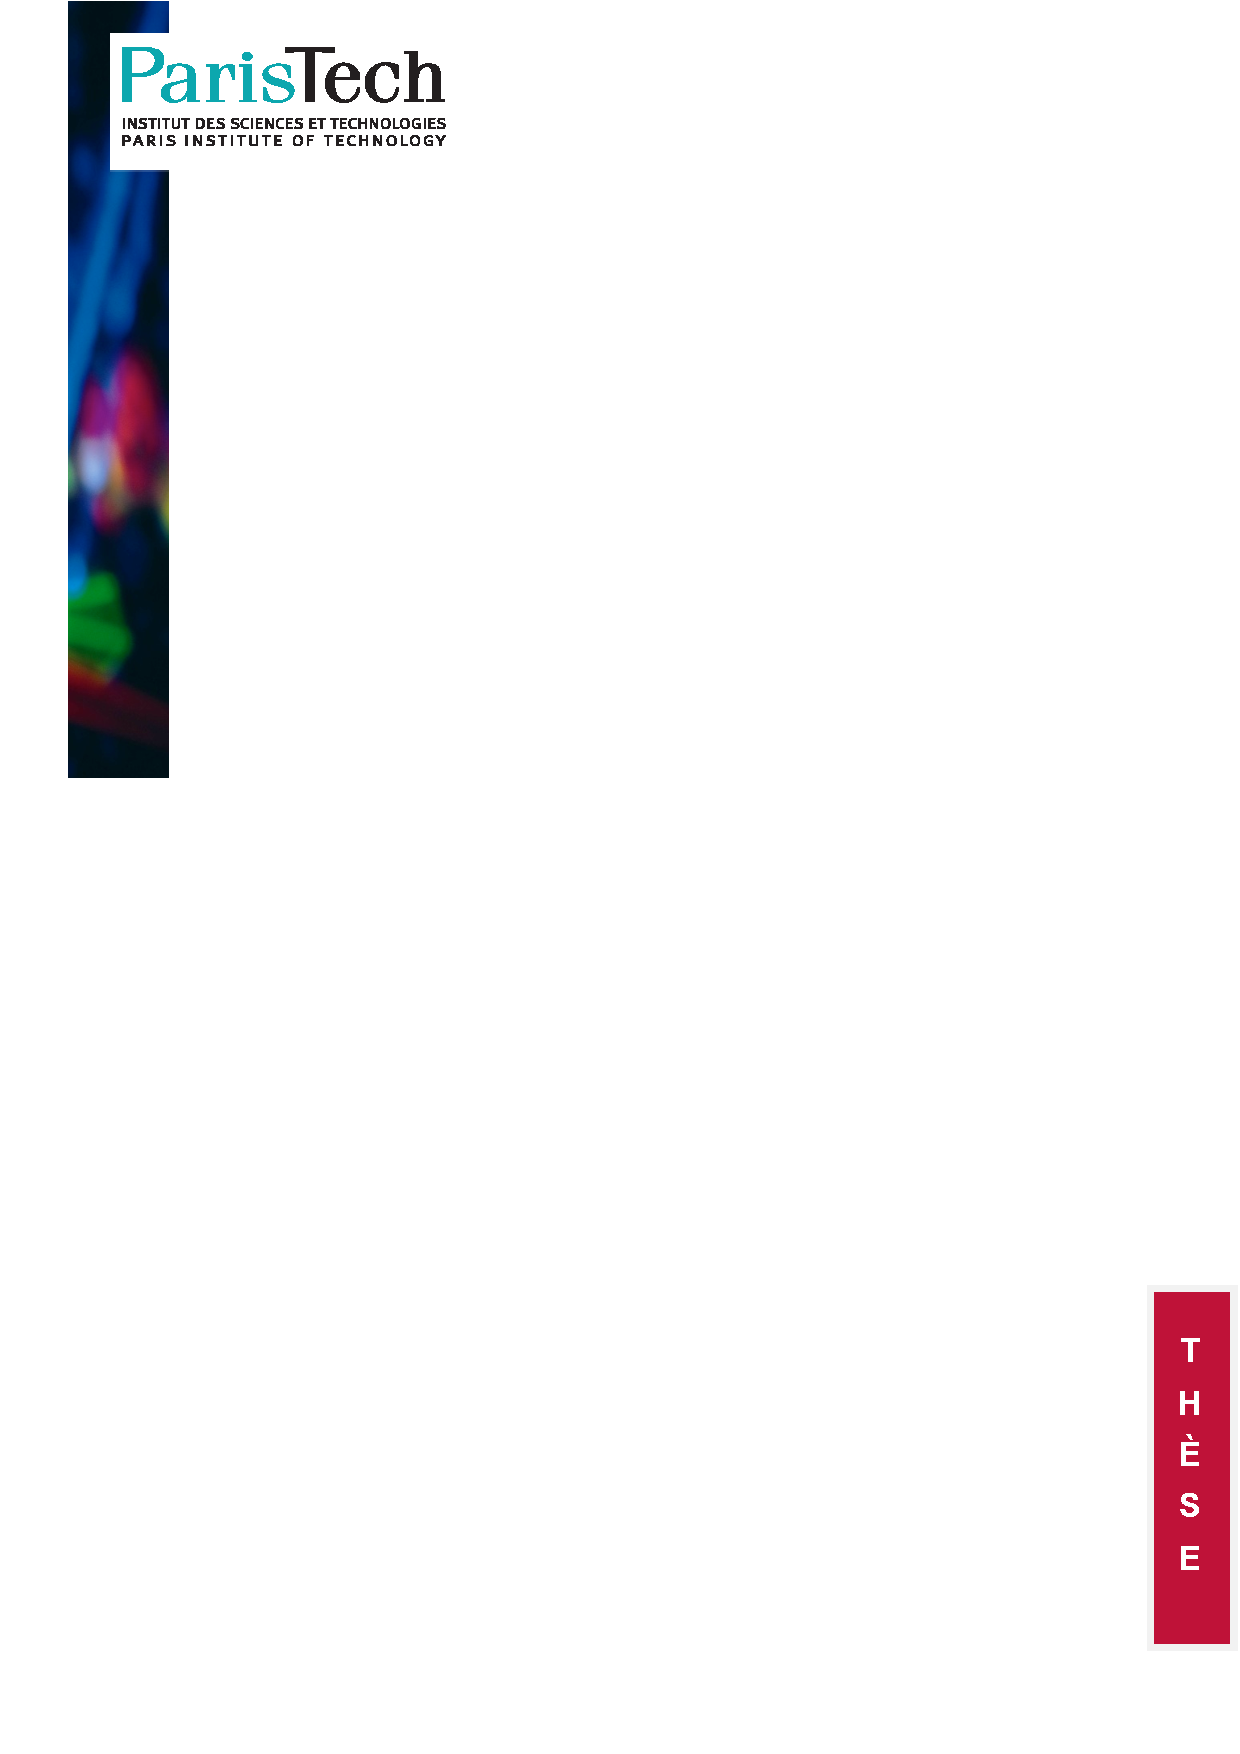
\includegraphics[height=\paperheight,width=\paperwidth]{img/logos/cover_bg.pdf}
\else
	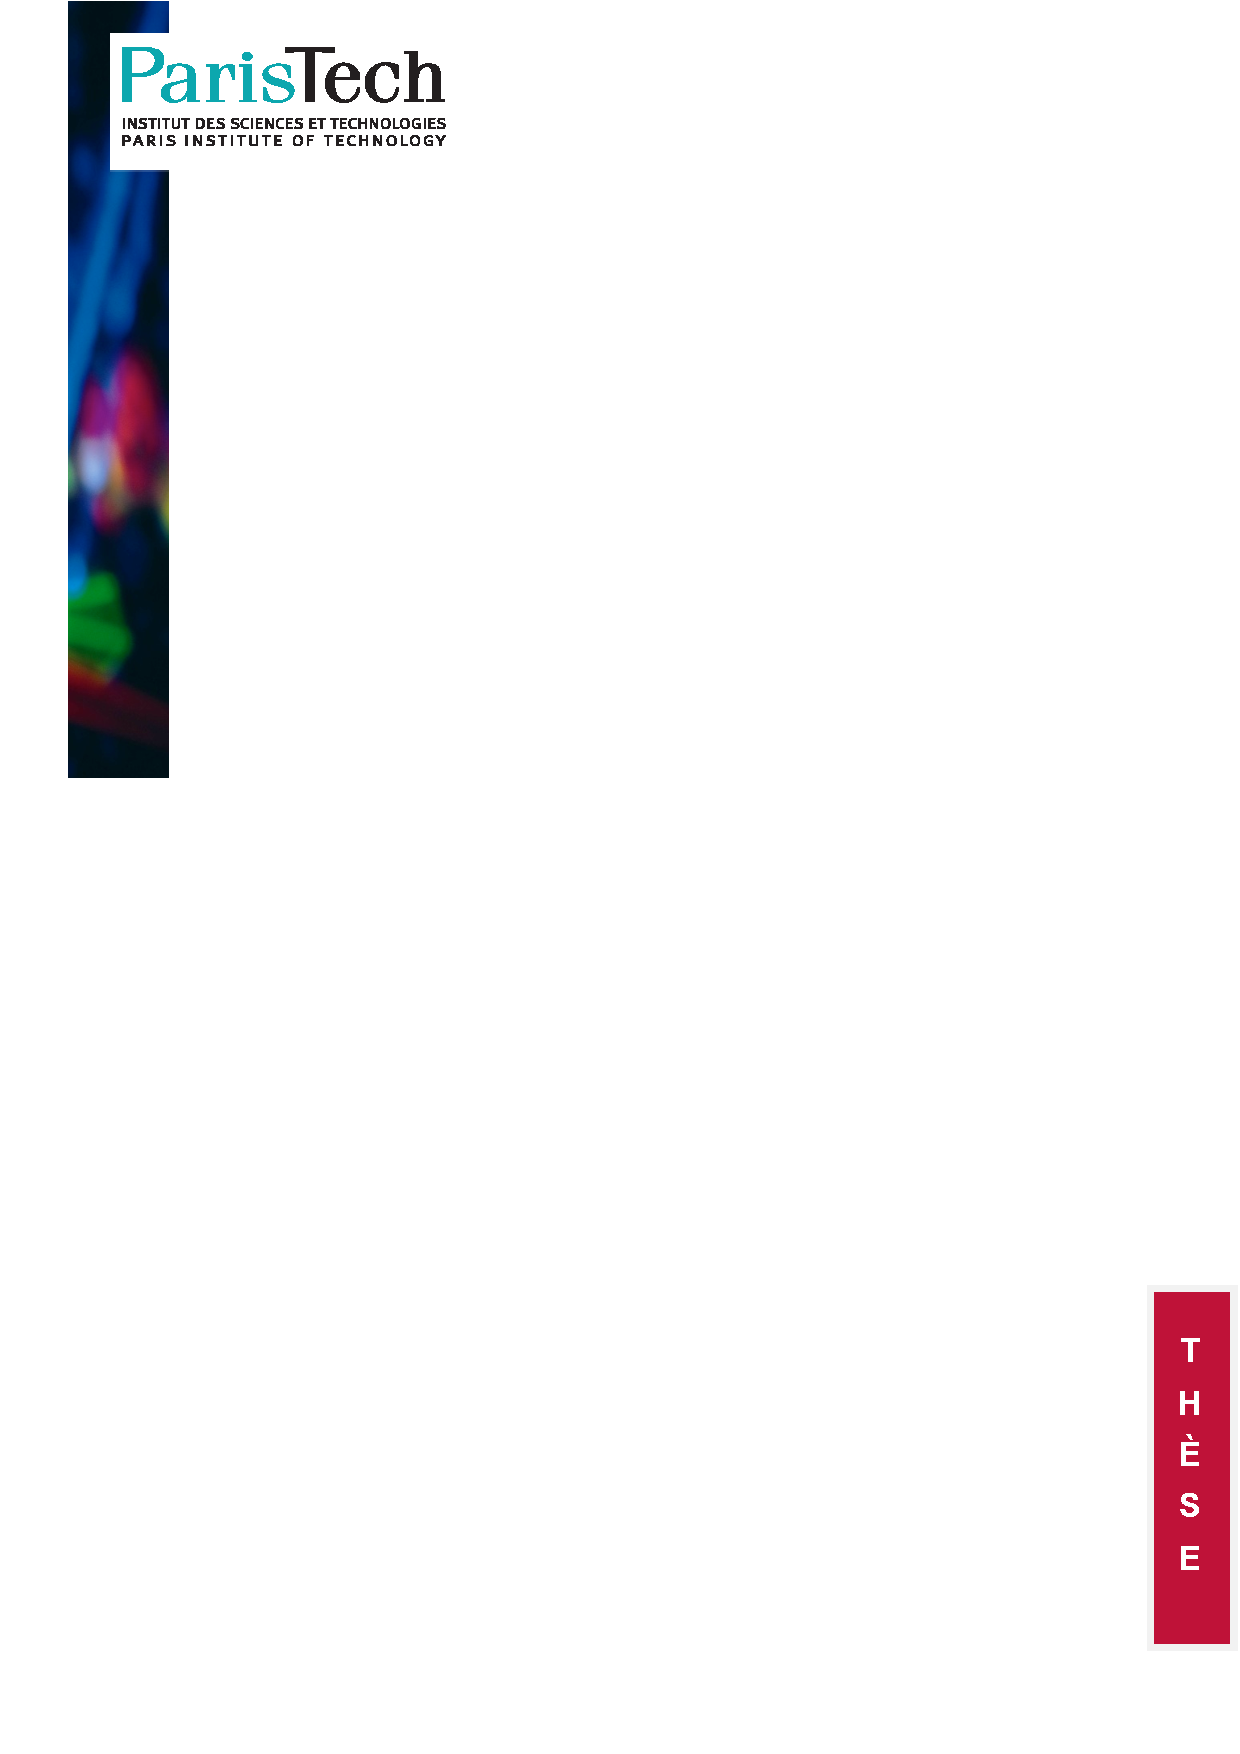
\includegraphics[height=\paperheight,width=\paperwidth]{img/logos/cover_bg.pdf}
\fi}

%----------------------------------------------------------------------------------------
%	FLOATS: TABLES, FIGURES AND CAPTIONS SETUP
%----------------------------------------------------------------------------------------

\usepackage{tabularx} % Better tables
\setlength{\extrarowheight}{3pt} % Increase table row height
\newcommand{\tableheadline}[1]{\multicolumn{1}{c}{\spacedlowsmallcaps{#1}}}
\newcommand{\myfloatalign}{\centering} % To be used with each float for alignment
\usepackage{caption}
\captionsetup{format=hang,font=small}
\usepackage{subcaption}


%----------------------------------------------------------------------------------------
%	BACKREFERENCES
%----------------------------------------------------------------------------------------

% \usepackage{ifthen} % Allows the user of the \ifthenelse command
% \newboolean{enable-backrefs} % Variable to enable backrefs in the bibliography
% \setboolean{enable-backrefs}{true} % Variable value: true or false

% \newcommand{\backrefnotcitedstring}{\relax} % (Not cited.)
% \newcommand{\backrefcitedsinglestring}[1]{(Cited on page~#1.)}
% \newcommand{\backrefcitedmultistring}[1]{(Cited on pages~#1.)}
% \ifthenelse{\boolean{enable-backrefs}} % If backrefs were enabled
% {
% \PassOptionsToPackage{hyperpageref}{backref}
% \usepackage{backref} % to be loaded after hyperref package 
% \renewcommand{\backreftwosep}{ and~} % separate 2 pages
% \renewcommand{\backreflastsep}{, and~} % separate last of longer list
% \renewcommand*{\backref}[1]{}  % disable standard
% \renewcommand*{\backrefalt}[4]{% detailed backref
% \ifcase #1 
% \backrefnotcitedstring
% \or
% \backrefcitedsinglestring{#2}
% \else
% \backrefcitedmultistring{#2}
% \fi}
% }{\relax} 

%----------------------------------------------------------------------------------------
%	CHANGING TEXT AREA 
%----------------------------------------------------------------------------------------

\usepackage[T1]{fontenc}
\usepackage[bitstream-charter]{mathdesign} % Font
\usepackage[Lenny]{fncychap} % Nice chapter headings Other choices : Sonny, Lenny, Glenn, Conny, Rejne, Bjarne

% DEBUG des subsubsection

\usepackage{minitoc} % Mini table of contents
\mtcselectlanguage{french} % Mini table of contents in French

\usepackage{epigraph} % This is to insert the nice quote at the beginning of the chapter 

%------------------------------------------------
% Page headers fancy style  
%------------------------------------------------

% TODO: Faire un joli header
\usepackage{fancyhdr}


\usepackage{tikz}
\usetikzlibrary{
  arrows,
  automata,
  backgrounds,
  calc,
  decorations.pathreplacing,
  fit,
  petri,
  positioning,
  shadows,
  shapes
}
\usepackage{tikz-timing}[2014/10/29]
\usetikztiminglibrary[rising arrows]{clockarrows}
\usepackage{xparse}


\definecolor{OliveGreen}{rgb}{0,0.6,0}

\usepackage{pifont}
\newcommand{\cmark}{\ding{51}}%
\newcommand{\xmark}{\ding{55}}%
\newcommand{\ok}{\raisebox{-1mm}{\textcolor{OliveGreen}{\Large$\checkmark$}}}
\newcommand{\bad}{\raisebox{-1mm}{\textcolor{red}{\Large\xmark}}}


\usepackage{titlesec}

\setcounter{secnumdepth}{4}

\titleformat{\paragraph}
{\normalfont\normalsize\bfseries}{\theparagraph}{1em}{}
\titlespacing*{\paragraph}
{0pt}{3.25ex plus 1ex minus .2ex}{1.5ex plus .2ex}


% Acronym package: Full name after each section / chapter
\usepackage{etoolbox}
%\preto\section\acresetall

% Commandes pour le cache et la supervision

\newcommand{\tx}{\textrm{Tx}}
\newcommand{\rx}{\textrm{Rx}}
\newcommand{\listen}{\mathcal{L}}
\newcommand{\sleep}{\mathcal{S}}
\newcommand{\req}{r}
\newcommand{\ans}{a}
\newcommand{\ack}{\textrm{ACK}}
\newcommand{\racine}{root}
\newcommand{\router}{router}
\newcommand{\server}{server}
\newcommand{\act}{A}
\newcommand{\cycle}{C}
\newcommand{\txtx}{\tx \to \tx}
\newcommand{\txrx}{\tx \to \rx}
\newcommand{\rxtx}{\rx \to \tx}
\newcommand{\rxrx}{\rx \to \rx}
\newcommand{\detect}{d}
\newcommand{\pkt}{p}
\newcommand{\cmin}{c_{min}}
\newcommand{\cmax}{c_{max}}
\newcommand{\copt}{c^*}


%----------------------------------------------------------------------------------------
% HYPERREFERENCES Should be the last package imported
%----------------------------------------------------------------------------------------

\PassOptionsToPackage{pdftex,hyperfootnotes=false,pdfpagelabels}{hyperref}
\usepackage{hyperref}  % backref linktocpage pagebackref
\pdfcompresslevel=9
\pdfadjustspacing=1

\hypersetup{
hypertexnames, % default is true since a long time
% Uncomment the line below to remove all links (to references, figures, tables, etc)
%draft, 
colorlinks=false, 
% linktocpage=true, 
pdfstartview=FitV,
% % Uncomment the line below if you want to have black links (e.g. for printing black and white)
% %colorlinks=false, linktocpage=false, pdfborder={0 0 0},
pdfstartview=FitV, 
% breaklinks=true, 
% pdfpagemode=UseOutlines,
% plainpages=false, 
% bookmarksnumbered, 
bookmarksopen=true,
% %urlcolor=webbrown, 
 linkcolor=RoyalBlue,
 citecolor=webgreen,
%------------------------------------------------
% PDF file meta-information
pdftitle={\myTitle},
pdfauthor={\textcopyright\ \myName, \myUni, \myFaculty},
pdfsubject={Passerelles pour réseaux contraints},
pdfkeywords={LLN, Low-Power and Lossy Networks, Wireless Sensors Networks},
pdfcreator={pdfLaTeX},
pdfproducer={LaTeX with hyperref}
% ------------------------------------------------
}